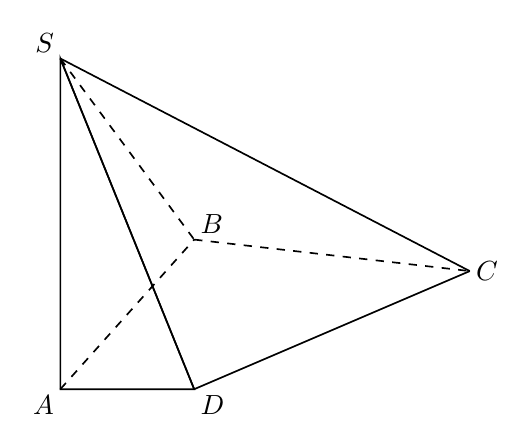
\begin{tikzpicture}[x=1cm,y=1cm,font=\normalsize,line width=.6pt]
\coordinate (S) at (0,4.2);
\coordinate (A) at (0,0);
\coordinate (D) at (1.7,0);
\coordinate (B) at (1.7,1.9);
\coordinate (C) at (5.2,1.5);
\draw[solid] (S) -- (A) -- (D) -- cycle;
\draw[solid] (S) -- (D);
\draw[solid] (D) -- (C);
\draw[solid] (S) -- (C);
\draw[dashed] (S) -- (B);
\draw[dashed] (A) -- (B);
\draw[dashed] (B) -- (C);
\node[above left,inner sep=2pt] at (S) {$S$};
\node[below left,inner sep=2pt] at (A) {$A$};
\node[below right,inner sep=2pt] at (D) {$D$};
\node[above right,inner sep=2pt] at (B) {$B$};
\node[right,inner sep=2pt] at (C) {$C$};
\end{tikzpicture}
